\section{Related Work}
\label{sec:related}
Our \ours estimates consistent 3D open-vocabulary semantics and seamlessly integrates with SLAM pipelines. Unlike previous methods that either use a closed set of categories, offline processing, 2D semantic representations or odometry. \cref{tab:sota} provides a comparative summary of recent related works based on these aspects, with further details discussed in the remainder of this section.

\boldparagraph{Open-Vocabulary Image Semantics.} 
The introduction of Contrastive Language-Image Pretraining (CLIP)~\cite{radford2021clip}, which encodes image and text tokens into a shared latent space, revolutionized semantic segmentation.
By computing similarity to text inputs, CLIP enables classification into any category expressible in language.
Several variations of CLIP have enhanced its performance~\cite{zhai2023siglip,  cherti2023openclip} and improved feature granularity, aiming to generate dense feature vectors~\cite{zhou2022extract, sun2024alpha} rather than per-image representations. 
While closed-vocabulary methods outperform on predefined sets, open-vocabulary offers optimization-free generalization, highly relevant for diverse applications.
\begin{comment}    
\boldparagraph{2D Open-Vocabulary from RGB and RGB-D.}
With the advent of Neural Radiance Fields (NeRFs)~\cite{mildenhall2021nerf} and 3D Gaussian Splatting (3DGS)~\cite{kerbl3Dgaussians}, semantics have become increasingly integrated into them.
LERF~\cite{lerf2023} embeds per-object multi-scale CLIP features within NeRF, enabling 2D image searches via language queries.
LangSplat~\cite{qin2024langsplat} applies the Segment Anything Model (SAM)~\cite{kirillov2023sam} on each viewpoint to generate 2D masks, remove their background, and encode them into CLIP vectors.
Features are then compressed into 3 channels and incorporated into a 3DGS~\cite{kerbl3Dgaussians} representation, allowing 2D semantic segmentation. 
Subsequent works build on LangSplat by incorporating affinity features optimized with a multi-view mask graph~\cite{cen2023saga} or by integrating both CLIP and DINOv2~\cite{oquab2023dinov2} features ~\cite{shi2024language,qiu-2024-featuresplatting}. 
The dependence of all these methods on multi-point 3D-2D transformations (via rendering or rasterization) for computing 2D semantic features limits their semantic representation to 2D--evidenced by the lack of proper 3D evaluation. 
\end{comment}
%


\boldparagraph{Offline 3D Open-Vocabulary from 3D point clouds.} Most open-vocabulary 3D semantic approaches assume a known 3D point cloud.
OpenScene~\cite{Peng2023OpenScene} leverages OpenSeg~\cite{ghiasi2022scaling} to compute CLIP features from images and trains a network to associate 2D pixels with 3D points.
For each 3D point it performs average pooling on CLIP vectors from multiple views and supervises an encoder to directly assign CLIP features to 3D point clouds. 
OpenMask3D~\cite{takmaz2023openmask3d} selects $k$ views per object, crops its 2D SAM mask to compute a CLIP features, and then features are average-pooled across crops and views. 
Open3DIS~\cite{nguyen2024open3dis} integrates SuperPoint~\cite{detone2018superpoint} with 2D instance segmentations and a 3D instance segmentator to generate multiple 3D instance proposals, describing each with CLIP features following OpenMask3D~\cite{takmaz2023openmask3d}.
In contrast, OpenYolo-3D~\cite{boudjoghra2024openyolo} uses a 2D open-vocabulary object detector instead of relying on 2D instance masks and CLIP features.
It classifies each object based on the most common class across all views.
While this approach eliminates the need for CLIP feature extraction, it limits each scene to a predefined set of classes.

\boldparagraph{Offline 3D Open-Vocabulary from RGB and RGB-D.} OpenNeRF~\cite{engelmann2024opennerf} optimizes a NeRF to encode the scene representation along with per-pixel CLIP features from OpenSeg. The OpenSeg features are projected into 3D to compute the mean and covariance of 3D points. The NeRF then renders novel views, prioritizing areas with high covariance to compute additional OpenSeg features and refine the model.
Hierarchical Open-Vocabulary 3D Scene Graphs (HOV-SG) \cite{hovsg} relies on an offline hierarchical global fusion approach that requires precomputing 3D segments and features for all frames. 
%HOV-SG first reconstructs the full point cloud from RGB+D data, using DBSCAN\cite{ester1996density} to filter noise.
These 3D segments and features are incrementally fused by merging observations across consecutive frames.
The authors argue that relying solely on masked segments, as in Concept-Graphs~\cite{gu2024conceptgraphs}, discards crucial contextual information. To address this, they propose a descriptor that merges in a handcrafted manner three CLIP embeddings per mask: (1) the full image, (2) the masked segment without background, and (3) the masked segment with background. We adopt this strategy, and contribute by proposing a novel approach to learn the CLIP merging operation.

\boldparagraph{Online Semantics.} To date, online semantic methods have focused mostly  on closed vocabularies. SemanticFusion~\cite{mccormac2017semanticfusion} was one of the first semantic SLAM pipelines, predicting per-pixel closed-set categories and fusing predictions from different views in 3D space. Fusion++~\cite{mccormac2018fusion++} uses Mask-RCNN~\cite{he2017mask} to initialize per-object Truncated Signed Distance Functions (TSDFs), building a persistent object-graph representation.
In contrast, PanopticFusion~\cite{narita2019panopticfusion} combines predicted instances and class labels (including background) to generate pixel-wise panoptic predictions, which are then integrated into a 3D mesh. More recent works, such as those by Menini et al.~\cite{menini2021real} and ALSTER~\cite{weder2023alster}, jointly reconstruct geometry and semantics in a SLAM framework.
Additionally, NIS-SLAM~\cite{zhai2024nis} trains a multi-resolution tetrahedron NeRF to encode color, depth and semantics. 
NEDS-SLAM~\cite{ji2024neds} is a 3DGS-based SLAM system with embedded semantic features to learn an additional semantic representation of a closed set of classes.
Similarly, Hi-SLAM~\cite{li2024hi} and SGS-SLAM~\cite{li2024sgs} augment a 3DGS SLAM with semantic ids of predefined set of classes. 
These approaches either assume known 2D ground-truth closed set of semantic classes (and therefore only tackle a multi-view fusion problem), or only represent 2D semantics, with limited capabilities for 3D segmentation or precise 3D object localization.
%
More recently, OpenFusion~\cite{yamazaki2024open} and Concept-Graphs~\cite{gu2024conceptgraphs} integrated open-vocabulary semantic descriptors into online 3D mapping pipelines. Concept-Graphs relies on the naive mask-cropping to compute CLIP descriptors, while OpenFusion uses SEEM~\cite{zou2023segment} and creates a TSDF with 3D segments. 
%O$_2$V-Mapping~\cite{tie20242} combines CLIP and SAM within NICE-SLAM~\cite{zhu2022nice} for an online reconstruction although only evaluating 2D semantics.
None of them, however, addresses the integration into a full SLAM pipeline with loop closure optimization as we do. % in this work.

\begin{table}[t]
  \scriptsize
  \caption{Overview of 3D semantic reconstruction baselines.}
  \label{tab:sota}
  \centering
  \setlength{\tabcolsep}{8pt} %{3pt} 
  \begin{tabular}{l c c c c }
    \toprule
     \multirow{2}{*}{Method}      & Open     & 3D   &  \multirow{2}{*}{Online}         & Loop \\
     & Vocabulary & semantics  & & Closure \\
    \midrule
    %LERF~\cite{lerf2023}                   & \cmark & \xmark & \xmark & -  \\
    %LangSplat~\cite{qin2024langsplat}      & \cmark & \xmark & \xmark  & -  \\
    OpenScene~\cite{Peng2023OpenScene}     & \cmark & \cmark & \xmark  & -  \\
    OpenMask3D~\cite{takmaz2023openmask3d} & \cmark & \cmark & \xmark  & - \\
    Open3DIS~\cite{nguyen2024open3dis}     & \cmark & \cmark & \xmark  & -  \\
    HOV-SG~\cite{hovsg}                    & \cmark & \cmark & \xmark & -  \\
    OpenNeRF~\cite{engelmann2024opennerf}  & \cmark & \cmark & \xmark  & -  \\
    \hdashline \noalign{\vskip 1pt}
    NEDS-SLAM~\cite{ji2024neds}            & \xmark & \xmark & \cmark  & \xmark \\
    NIS-SLAM~\cite{zhai2024nis}            & \xmark & \xmark & \cmark  & \xmark  \\
    SGS-SLAM~\cite{li2024sgs}            & \xmark & \cmark & \cmark  & \xmark  \\
    Kimera-VIO~\cite{rosinol2020kimera}    & \xmark & \cmark & \cmark & \xmark  \\ \hdashline
    Concept-Fusion~\cite{conceptfusion}        & \cmark & \cmark & \cmark  & \xmark  \\
    Concept-Graphs~\cite{gu2024conceptgraphs}        & \cmark & \cmark & \cmark  & \xmark  \\
    Open-Fusion~\cite{yamazaki2024open}        & \cmark & \cmark & \cmark  & \xmark  \\
    \hdashline \noalign{\vskip 1pt}
    \textbf{\ours (ours)}             & \cmark & \cmark & \cmark & \cmark \\
    \bottomrule
  \end{tabular}
\end{table}
\begin{figure*}[ht!]
    \centering
    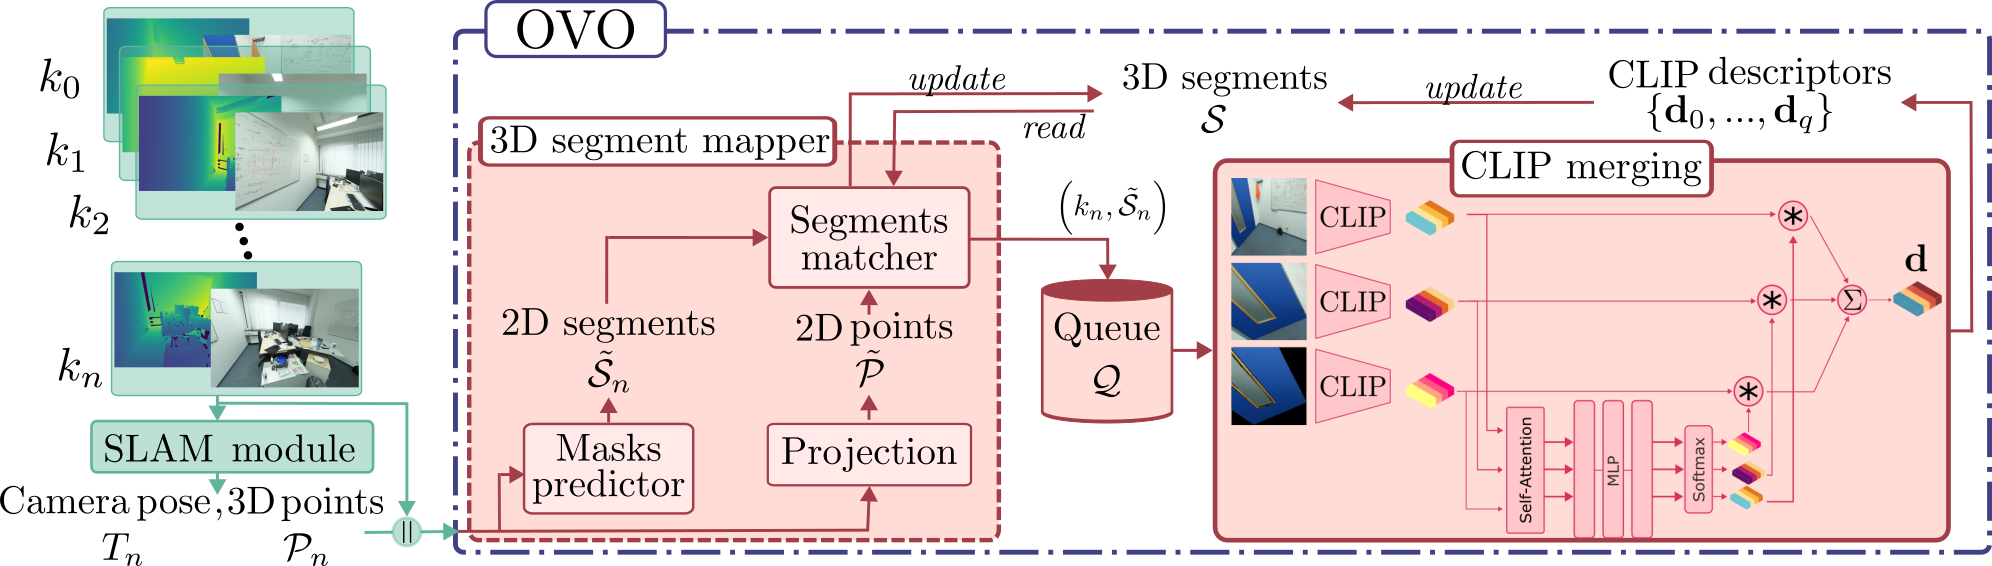
\includegraphics[width=\linewidth]{figures/images/ovomapping.png}
    \caption{\textbf{Overview.} From a stream of RGB-D keyframes, \ours builds, online, a 3D semantic representation of the scene. It relies on a 3D segment mapper to cluster 3D points into 3D segments; a queue to distribute the CLIP extraction computation, and a novel CLIP merging method to aggregate CLIP descriptors from multiple keyframes into one for each 3D segment.}
    \label{fig:ovo}
\end{figure*}